O registro fotográfico das visitas de campo consolidou a base empírica do diagnóstico participativo em duas localidades de referência, Baixão da Tranqueira em 19 de agosto de 2026 e Baixão de Cima em 10 de setembro de 2026, cujos sistemas e práticas documentados sustentam a derivação do bloco suplementar. O acervo organiza-se em torno da pactuação coletiva e da transmissão oral, da leitura da topossequência e do regime hídrico, do portfólio produtivo de microatividades, da farmacopeia local, das expressões devocionais e da memória territorial da ocupação, e o quadro exemplificativo (Tabela~\ref{tab:quadro_localidades}) associa cada registro à dimensão de vulnerabilidade biocultural e ao campo correspondente do instrumento.

\begin{table}[H]
\centering
\caption{Registros de campo nas localidades de referência, com correspondência entre o sistema documentado, a dimensão de vulnerabilidade biocultural e o campo do instrumento.}
\label{tab:quadro_localidades}
\small
\setlength{\tabcolsep}{4pt}
\begin{tabular}{p{3.4cm}p{4.4cm}p{1.3cm}p{3.9cm}}
\toprule
\textbf{Localidade e data} & \textbf{Sistema e registro documentado} & \textbf{Dim.} & \textbf{Campo correspondente do instrumento} \\
\midrule
Baixão da Tranqueira, 19/08/2026 & Roda intergeracional e plenária com depoimento de mestre de saberes, registradas em áudio e vídeo & $V_1$, $V_5$ & §6.1 Impactos socioculturais; protocolo de pactuação pré-oficina \\
\addlinespace
Baixão da Tranqueira, 19/08/2026 & Travessia conduzida por mestra sobre laje arenítica, com neossolo litólico e afloramentos expostos & $V_2$, $V_8$ & §5 Ambiente natural; §2 Descrição \\
\addlinespace
Baixão da Tranqueira, 19/08/2026 & Afloramento de neossolo litólico na topossequência, com mandacaru sobre solo raso & $V_2$, $V_8$ & §5 Ambiente natural \\
\addlinespace
Baixão da Tranqueira, 19/08/2026 & Capote (caldeirão escavado na rocha), reserva hídrica sazonal de acesso comunitário & $V_2$, $V_8$ & §5.9 Infraestrutura; §3 Classificação \\
\addlinespace
Baixão da Tranqueira, 19/08/2026 & Roçado consorciado de banana e citros, com urucum de uso medicinal e corante no quintal & $V_1$, $V_7$ & §2 Descrição; §4 Insumos e custos \\
\addlinespace
Baixão de Cima, 10/09/2026 & Imagem da padroeira com fitas votivas sobre esteira, na capela comunitária & $V_1$, $V_2$ & §6.1 Impactos socioculturais \\
\addlinespace
Baixão de Cima, 10/09/2026 & Sulco de erosão linear na trilha de acesso ao povoado & $V_8$ & §5 Ambiente natural, degradação \\
\addlinespace
Baixão de Cima, 10/09/2026 & Barreiro de reserva hídrica sazonal de uso comunitário & $V_5$, $V_8$ & §5.9 Infraestrutura; §5.6 Características dos usuários \\
\addlinespace
Baixão de Cima, 10/09/2026 & Percurso no escarpamento arenítico, com licurizeiras sob estiagem & $V_2$, $V_8$ & §5 Ambiente natural \\
\addlinespace
Baixão de Cima, 10/09/2026 & Cerca de estacas com quintal de mandioca & $V_2$, $V_5$ & §2 Descrição; §5.9 Infraestrutura \\
\bottomrule
\end{tabular}
\fonte{\textbf{Elaborado pelos autores} (2026), a partir do acervo fotográfico e audiovisual das visitas de campo.}
\end{table}

Os registros distribuíram-se segundo a cobertura que cada localidade ofereceu às oito dimensões, com Baixão da Tranqueira concentrando a evidência geológica, hídrica e de consorciação produtiva e Baixão de Cima contribuindo com a expressão devocional, o escarpamento arenítico e o quintal de mandioca. O painel fotográfico (Figura~\ref{fig:registros_campo}) reúne as categorias que o núcleo do WOCAT-SLM registra sem perda, como o afloramento litólico, os capotes e a consorciação de culturas, ao lado das categorias que exigiram bloco suplementar, como a farmacopeia de plantas de uso medicinal e a devoção à padroeira.

\begin{figure}[H]
\centering
\begin{minipage}{0.24\textwidth}
\centering
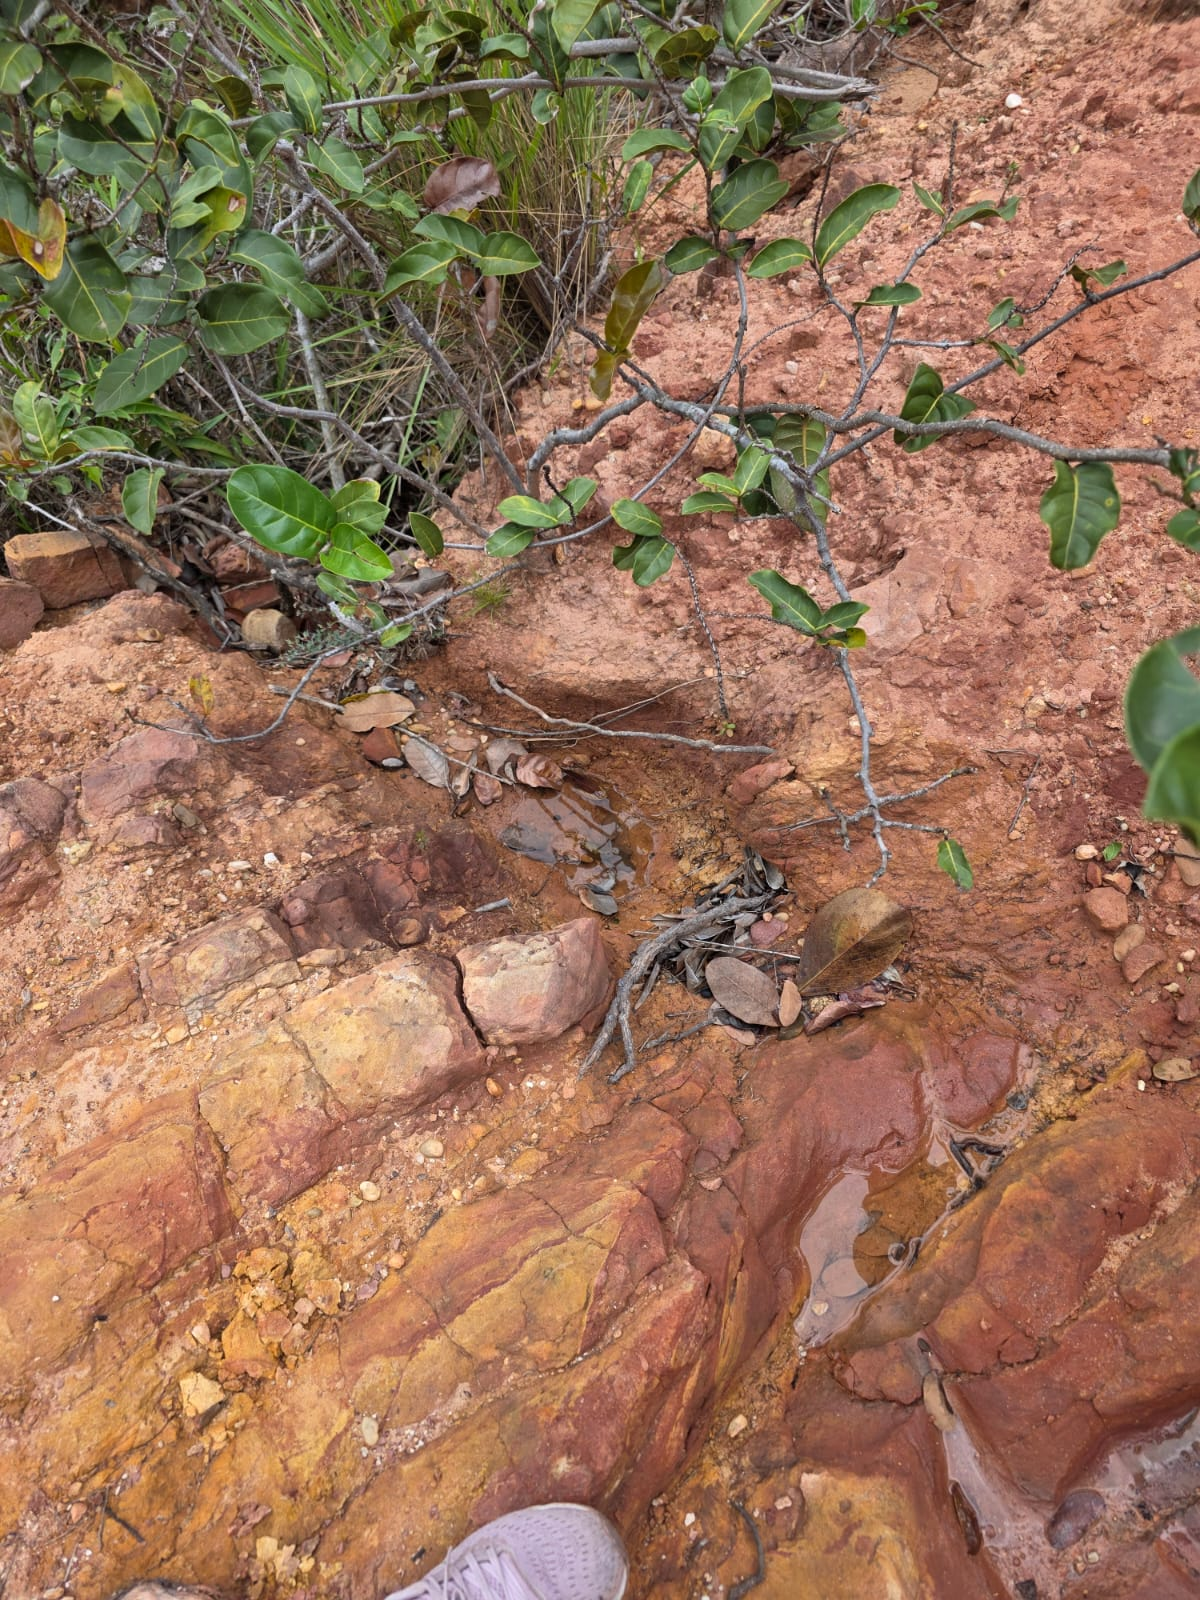
\includegraphics[width=\textwidth]{FIGURAS/visitas_campo/tranqueira_20260819_15_neossolo_litolico_afloramento.jpg}
\end{minipage}\hfill
\begin{minipage}{0.24\textwidth}
\centering
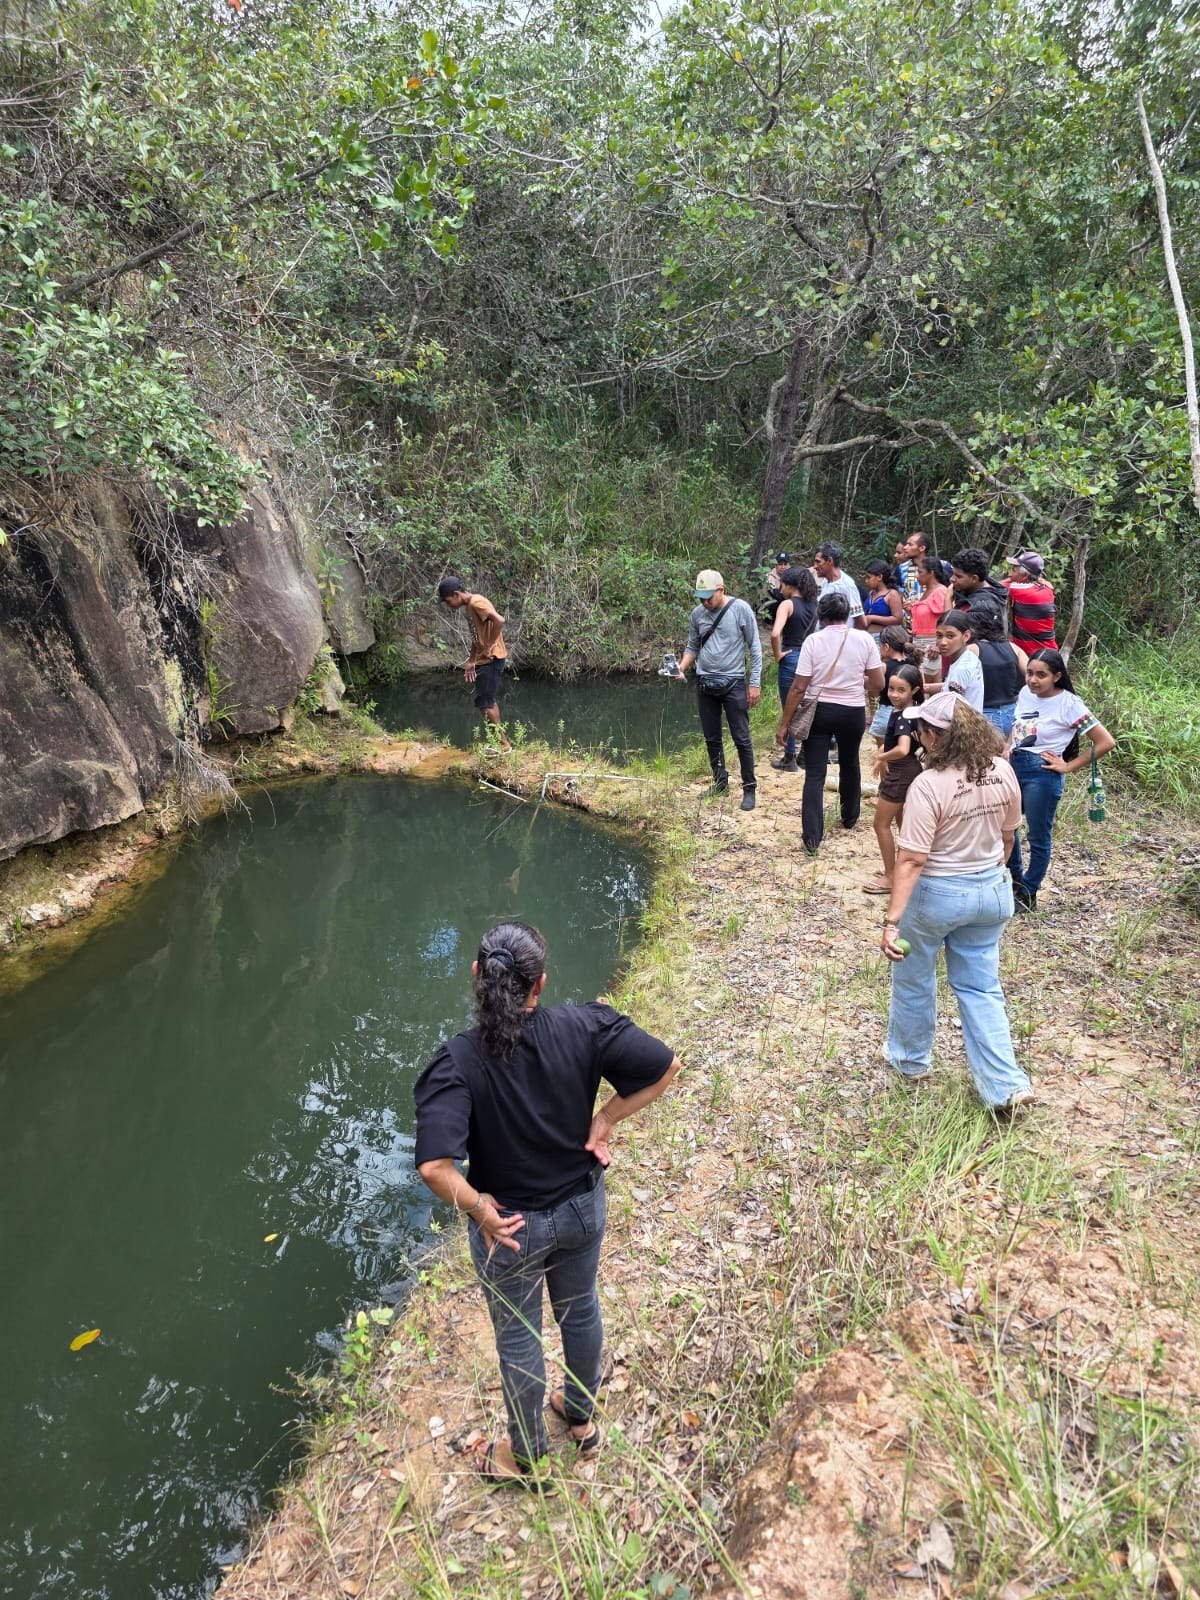
\includegraphics[width=\textwidth]{FIGURAS/visitas_campo/tranqueira_20260819_17_caldeirao_reserva_hidrica.jpg}
\end{minipage}\hfill
\begin{minipage}{0.24\textwidth}
\centering
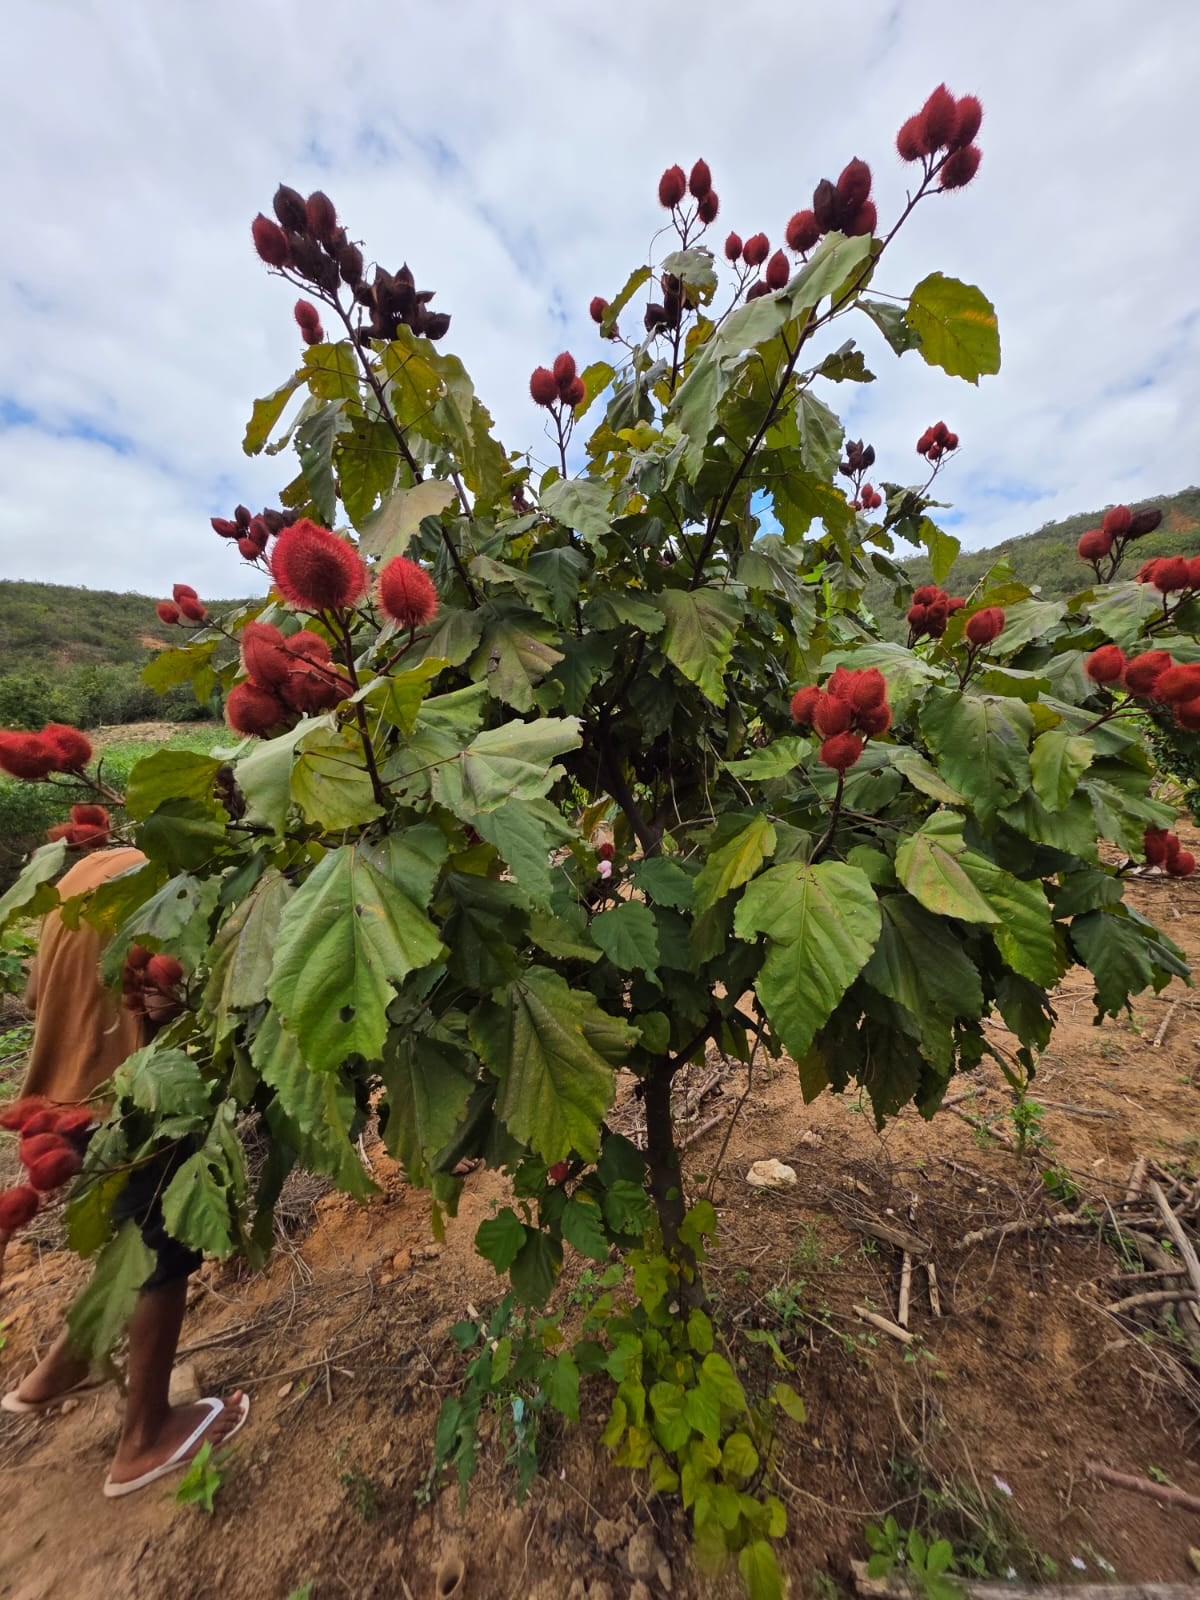
\includegraphics[width=\textwidth]{FIGURAS/visitas_campo/tranqueira_20260819_18_urucum_bixa_orellana.jpg}
\end{minipage}\hfill
\begin{minipage}{0.24\textwidth}
\centering
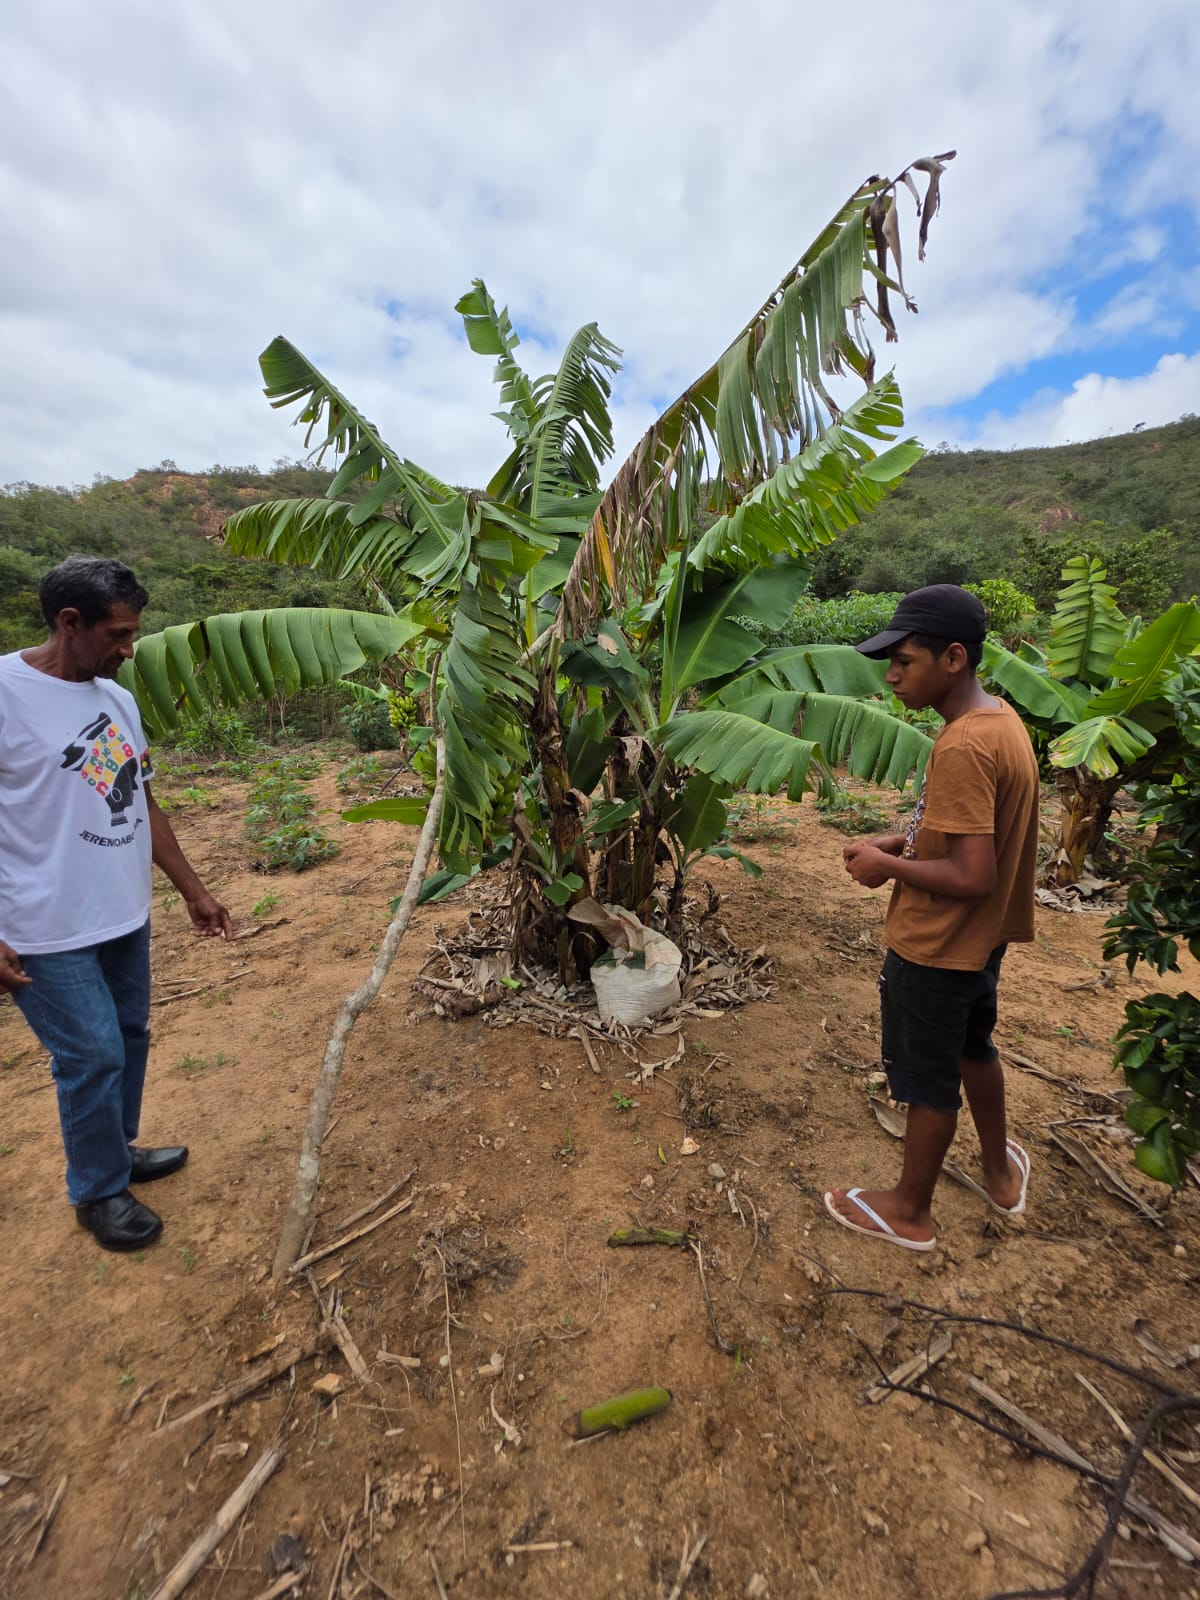
\includegraphics[width=\textwidth]{FIGURAS/visitas_campo/tranqueira_20260819_19_rocado_consorciado_banana_citros.jpg}
\end{minipage}

\vspace{0.5em}

\begin{minipage}{0.24\textwidth}
\centering
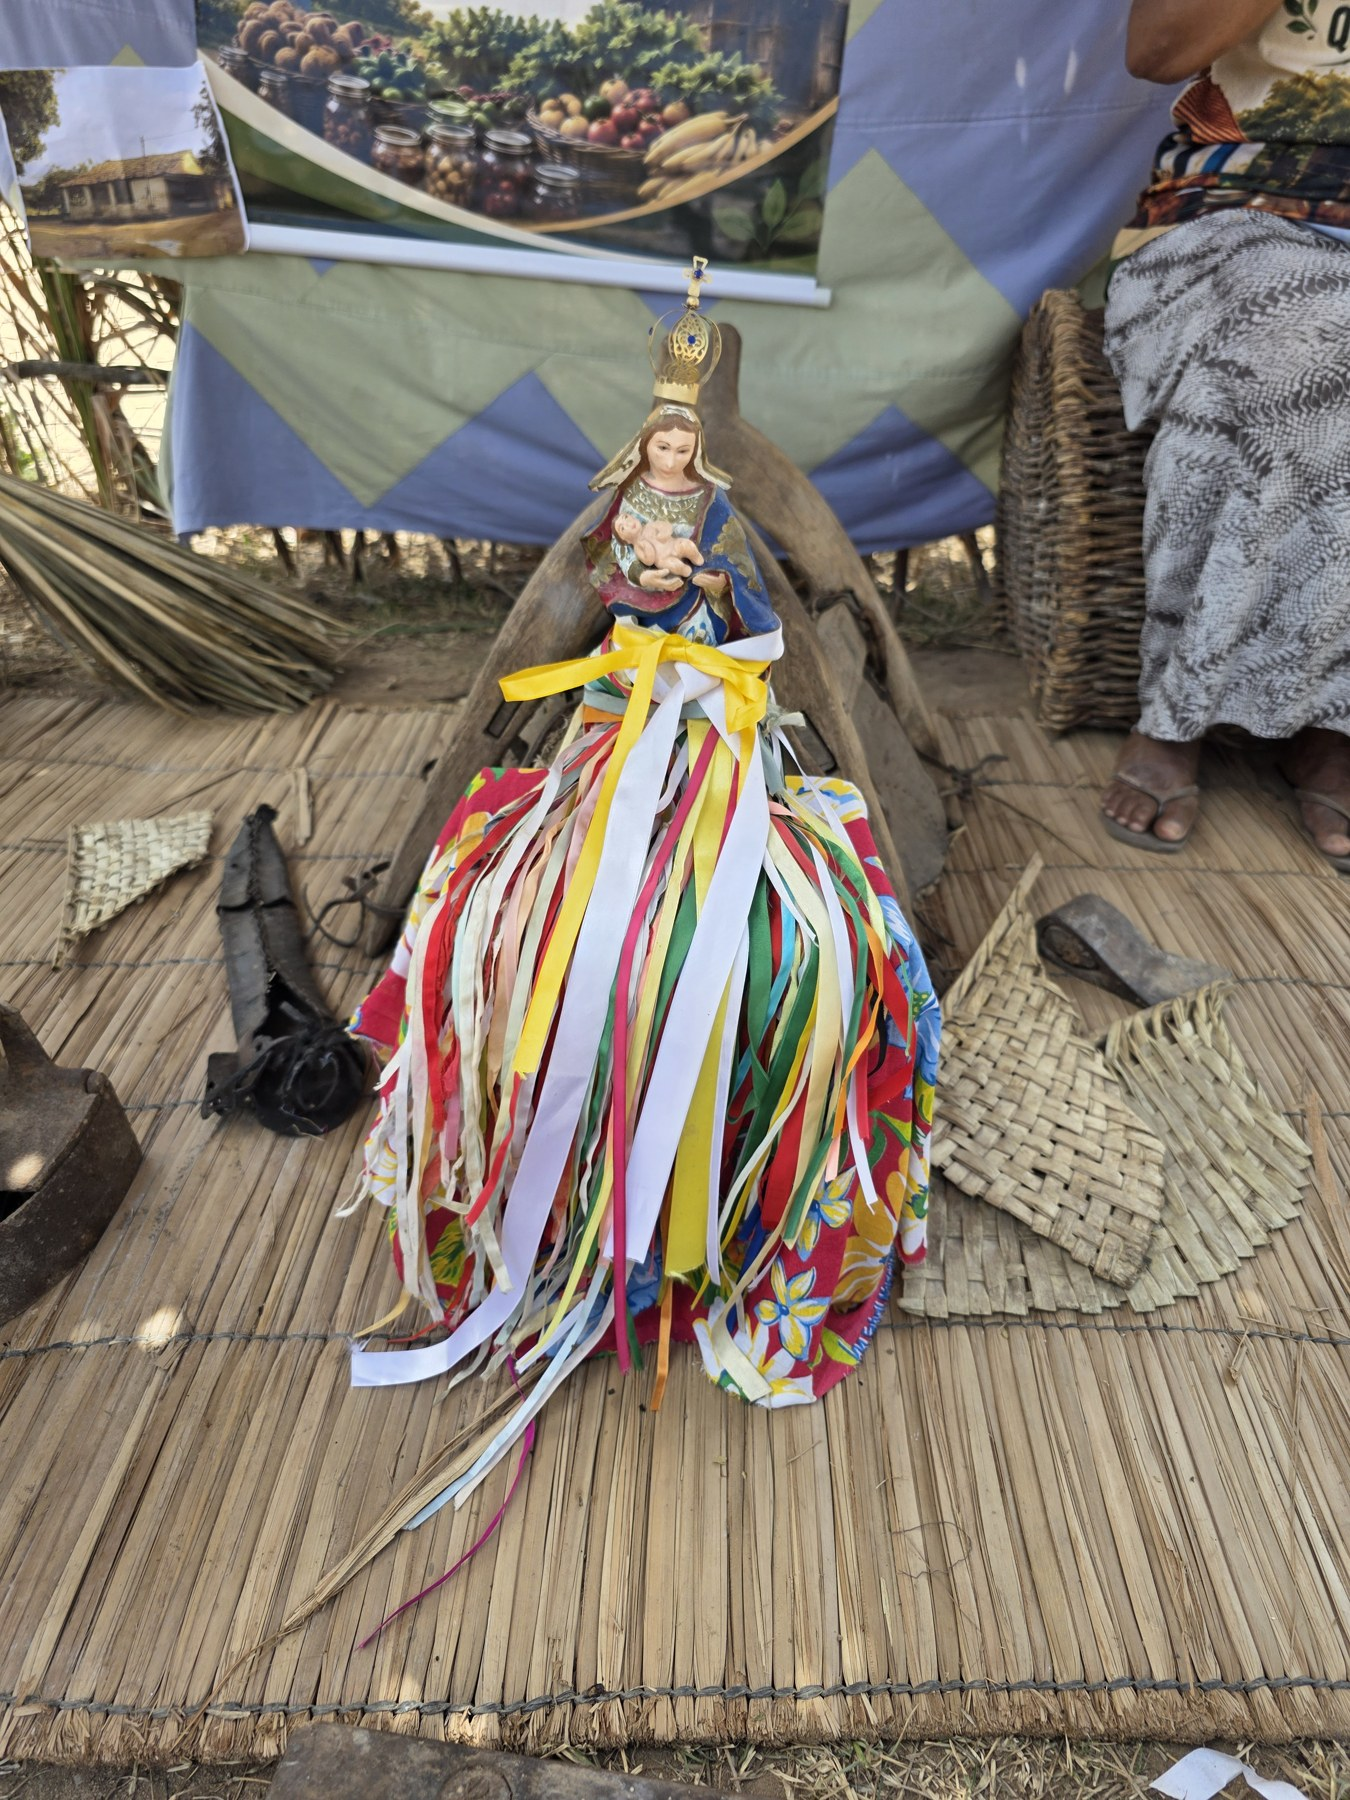
\includegraphics[width=\textwidth]{FIGURAS/visitas_campo/baixao_de_cima_20260910_02_imagem_padroeira_fitas_sobre_esteira.jpg}
\end{minipage}\hfill
\begin{minipage}{0.24\textwidth}
\centering
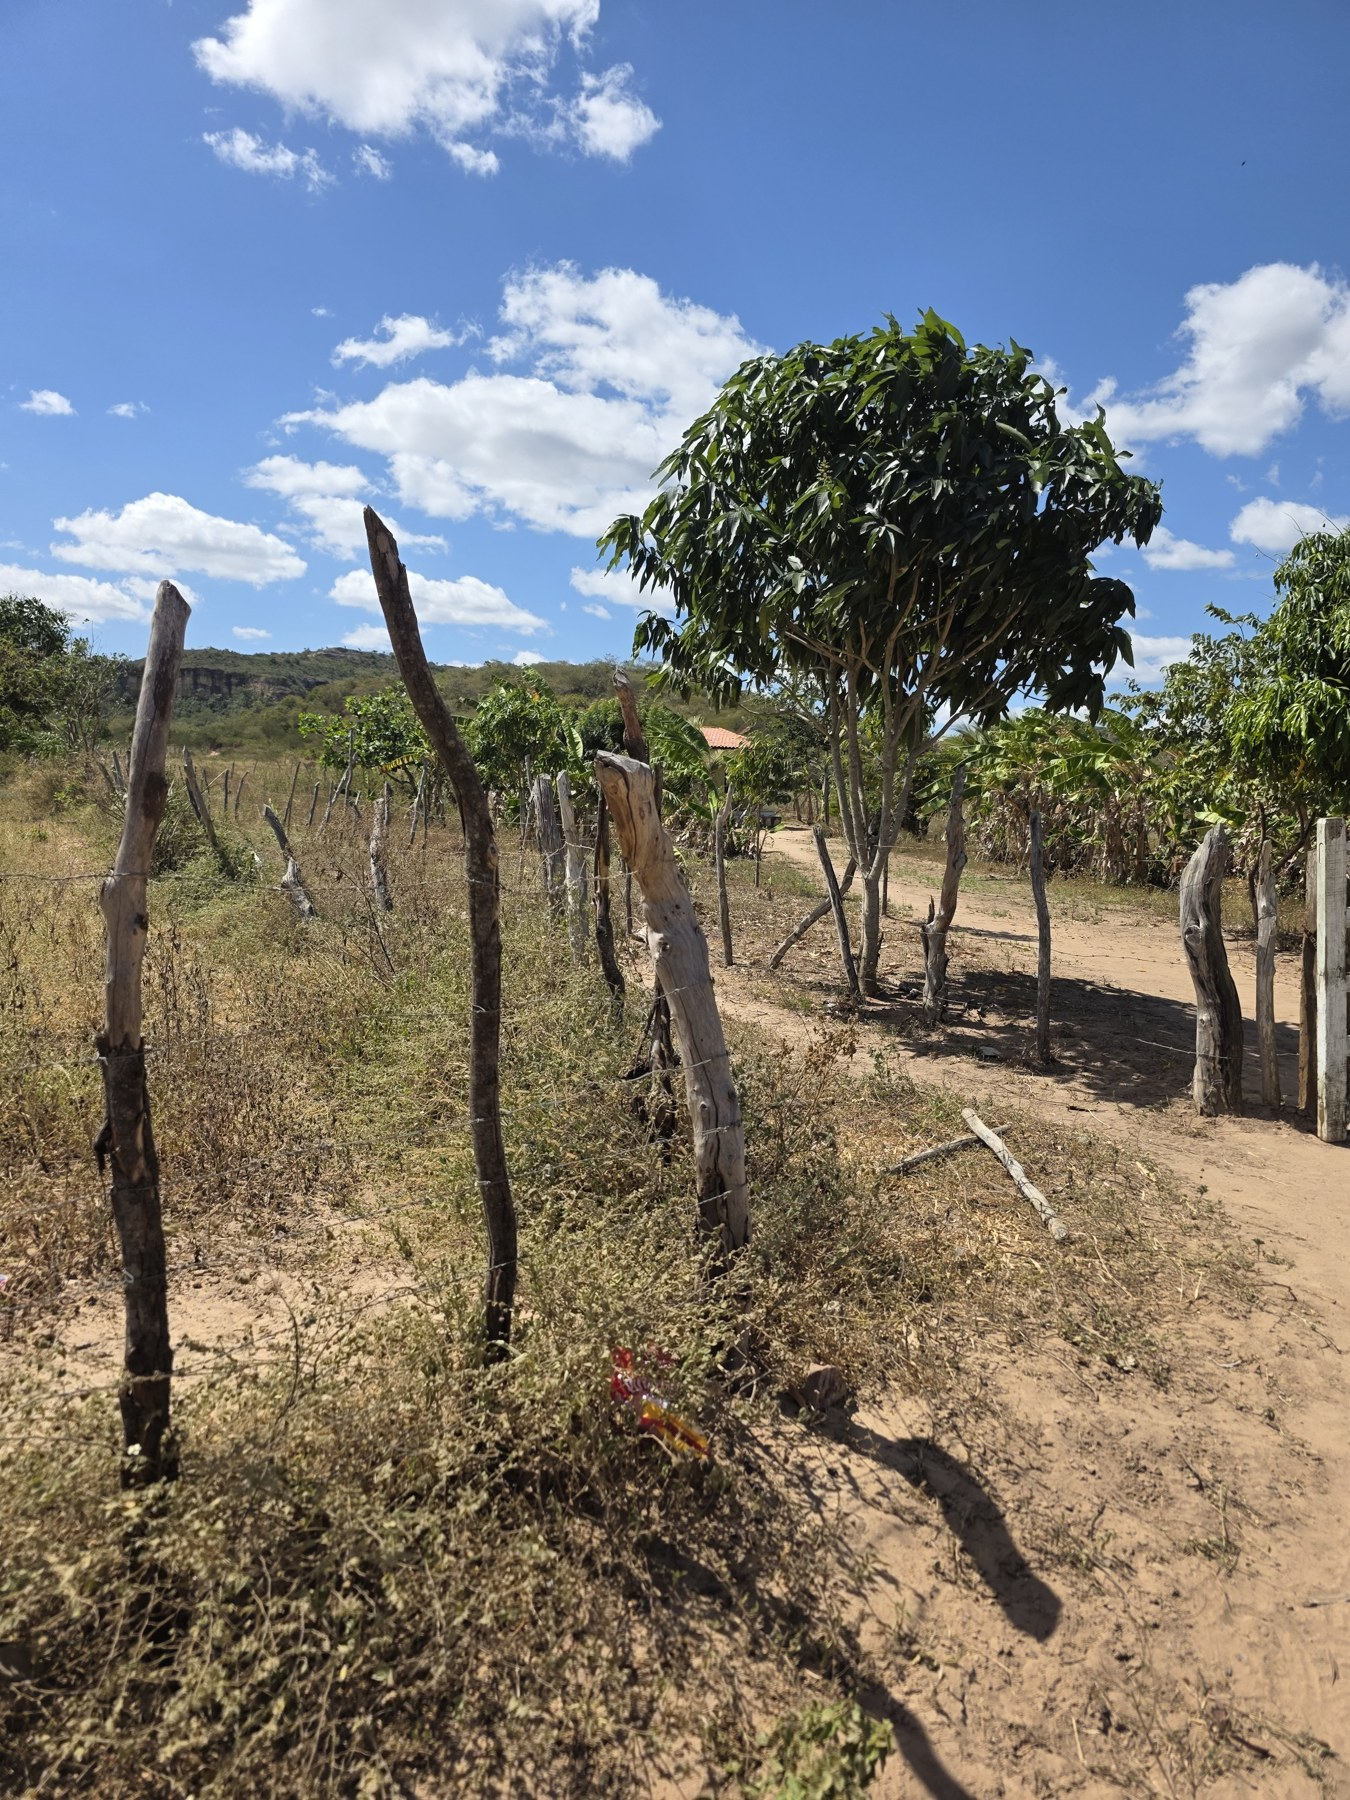
\includegraphics[width=\textwidth]{FIGURAS/visitas_campo/baixao_de_cima_20260910_10_cerca_estacas_quintal_mandioca.jpg}
\end{minipage}\hfill
\begin{minipage}{0.24\textwidth}
\centering
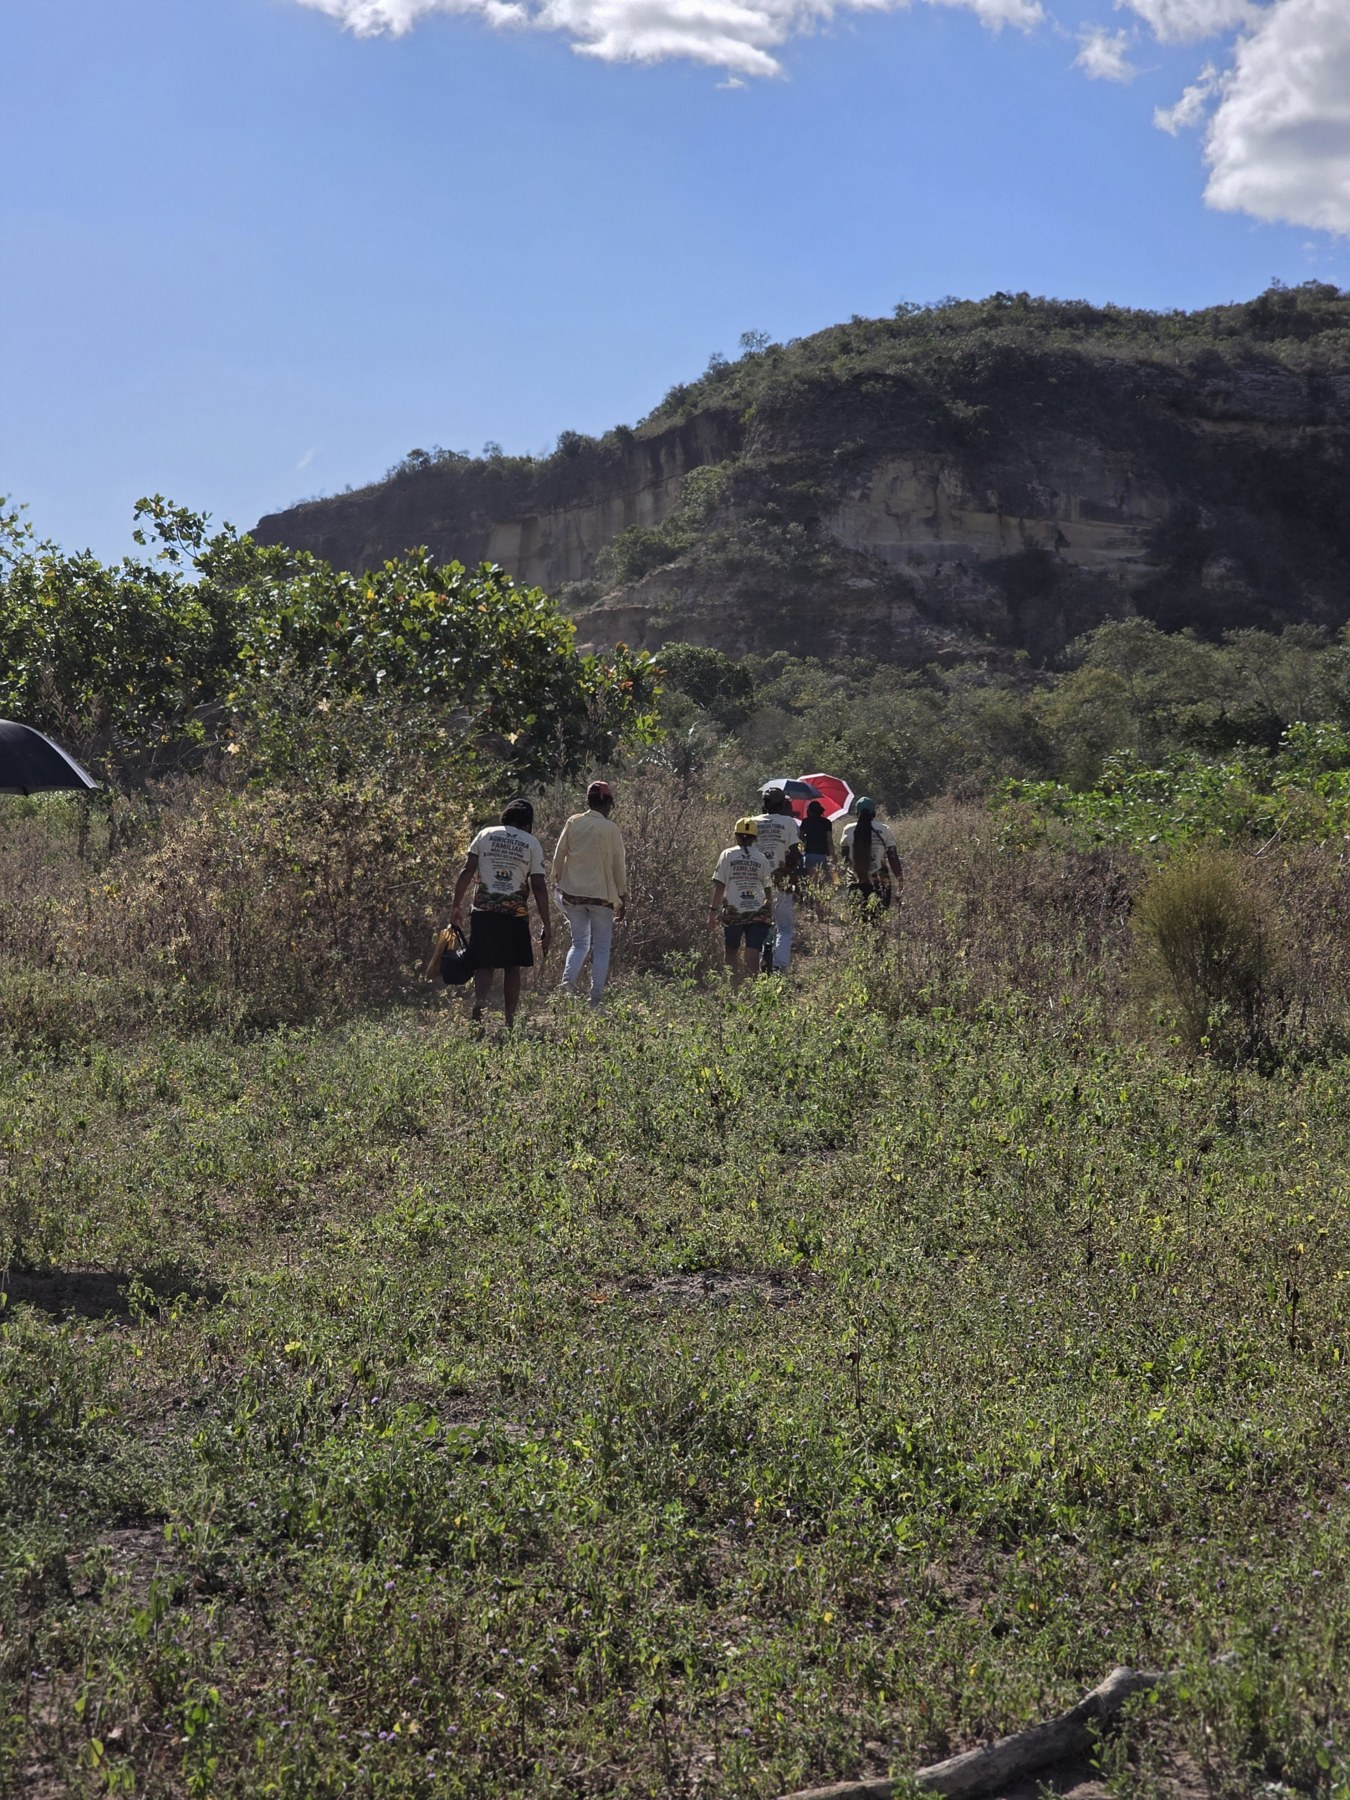
\includegraphics[width=\textwidth]{FIGURAS/visitas_campo/baixao_de_cima_20260910_13_percurso_escarpamento_arenitico.jpg}
\end{minipage}\hfill
\begin{minipage}{0.24\textwidth}
\centering
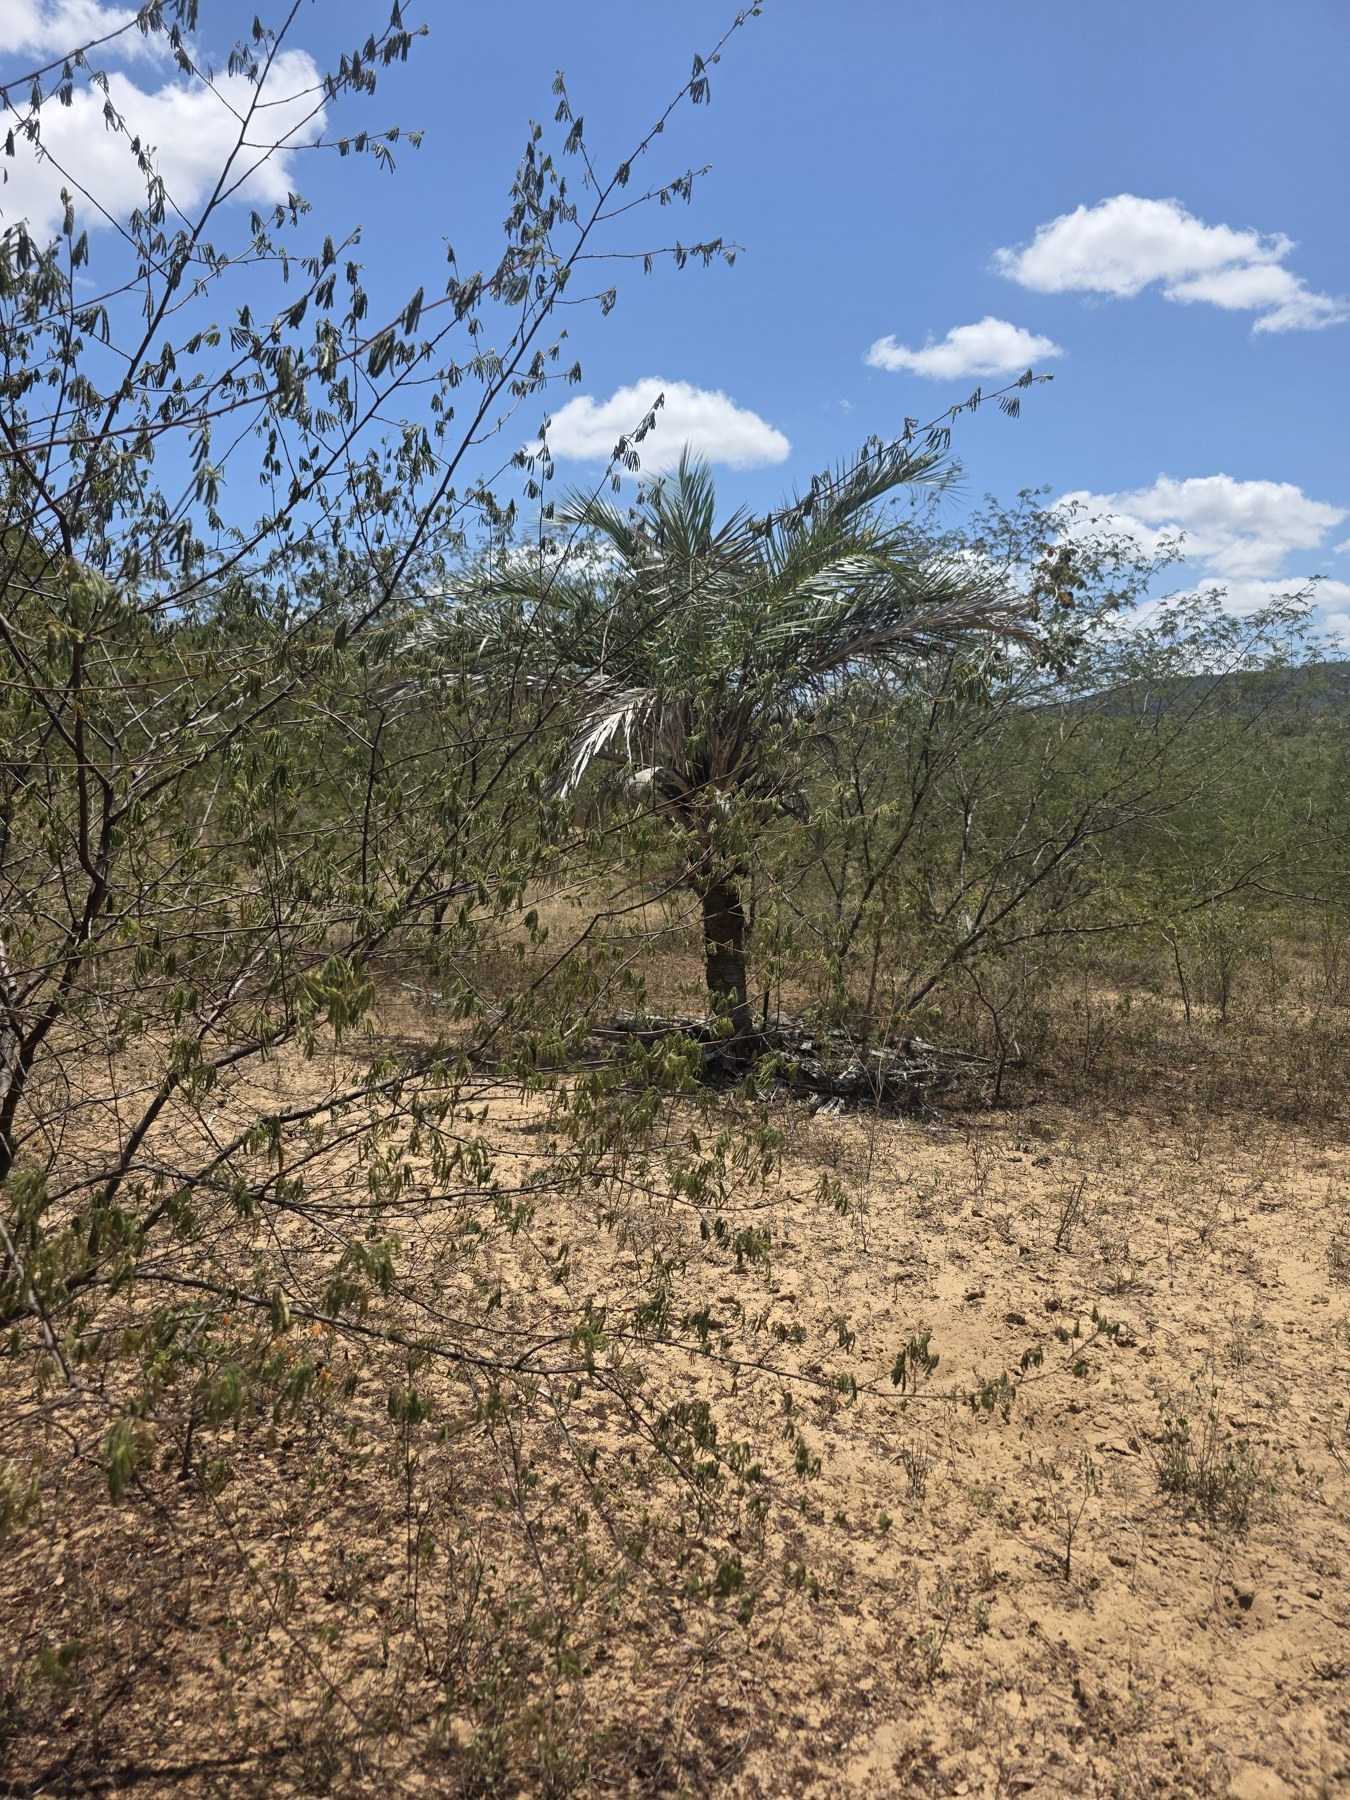
\includegraphics[width=\textwidth]{FIGURAS/visitas_campo/baixao_de_cima_20260910_04_caatinga_licurizeira_estiagem.jpg}
\end{minipage}
\caption{Registros fotográficos das localidades de referência em Baixão da Tranqueira (afloramento de neossolo litólico, capote, urucum e roçado consorciado) e em Baixão de Cima (imagem da padroeira, quintal de mandioca, escarpamento arenítico e licurizeiras em estiagem). Fonte: acervo dos autores (2026).}
\label{fig:registros_campo}
\end{figure}
